% !TeX root = ../main.tex

\chapter{Teoria da informação em análise de formas \label{chap:TINFO}}

Neste capítulo apresentamos conceitos da teoria da informação que são utilizados na proposta de descrição multiescala de formas e na avaliação de similaridade das mesmas.
Para tanto apresentamos a entropia de Shannon e a entropia diferencial, bem como suas propriedades. Em seguida as medidas de divergência que foram utilizadas na análise de similaridade de formas. Então descrevemos a metodologia utilizada para obtenção de descritores de forma a partir da entropia diferencial para finalmente apresentarmos a metodologia utilizada para a análise de similaridade de formas através de divergentes e assinaturas de formas.

\section{Conceitos da teoria da informação}

Conceitos da teoria da informação têm sido aplicados, recentemente e com sucesso, em problemas de visão computacional e reconhecimento de padrões. Isso porque tais conceitos têm se mostrado apropriados para a modelagem do comportamento dos sistemas biológicos de percepção visual \cite{Escolano:2009}.

Grandezas como entropia e informação mútua também tem sido utilizadas como função custo no treinamento de sistemas adaptativos e de aprendizagem de máquina \cite{Principe:2011} pelo fato de terem relação direta com a informação contida nos sinais. Essas grandezas são expressas pelas funções densidade de probabilidade dos dados, que portanto devem ser estimadas. 

\subsection{Entropia de Shannon}

Na teoria da informação, a entropia de Shannon é uma medida do grau de incerteza que se tem, em média, dos possíveis estados que uma variável aleatória discreta pode assumir. Seja  $X$ uma variável aleatória discreta, que possa assumir $N$ diferentes valores $\{x_1\text{, } \ldots\text{ , }x_k\text{ , }\ldots\text{ , }x_N$\}, aonde a probabilidade de ocorrência de cada valor é $p_k = P(X = x_k) \text{,} \quad 0 \leq p_k \leq 1 \text{,} \quad \sum \limits_{k=1}^N p_k = 1$. A entropia de Shannon de $X$ é definida pela seguinte equação 

\begin{equation}\label{eq:Shannon}
H(X) = -\sum\limits_{k = 1}^N p_k\log{p_k}
\end{equation}

e apresenta as seguintes propriedades \cite{Thomas:2006}:

\begin{alineas}
\item $0 \leq H(X) \leq \log{N}$;  
\item $H(X) = 0$ se $p_k = 1$ para um único valor de $k$ e $p_k = 0$ para os demais valores de $k$;
\item $H(X) = \log{N}$ se $p_k = \frac{1}{N}$ para todos os valores de $k$.
\end{alineas}

A entropia de Shannon indica, em média, quanto de informação uma variável aleatória carrega. Quanto mais informativa uma variável aleatória é, maior o grau de surpresa que esta apresenta, ou seja, menos previsível é o seu valor.

\subsection{Entropia diferencial}

Para uma variável aleatória contínua $X$, com função densidade de probabilidade $p_X(x)$, a entropia diferencial é definida como sendo \cite{Thomas:2006}

\begin{equation}\label{eq:difent}
h(X) = -\int_{-\infty}^\infty p_X(x)\log{p_X(x)}dx\text{.}
\end{equation}

Essa definição é a extensão da entropia discreta de Shannon para o caso de variáveis aleatórias contínuas. No entanto, diferente da entropia de Shannon, a entropia diferencial não mede o grau de incerteza de $X$, pois tal incerteza é infinita, já que a quantidade de estados que um sistema contínuo pode realizar é infinita.

Considerando que uma variável aleatória contínua é o caso limite da variável aleatória discreta $X$, que assume valores $x_k = k \delta x$, $k = 0\text{, }\pm 1\text{, } \pm 2\text{, }\ldots$, quando $\delta x \mapsto 0$, demonstra-se que $H(X)$ e $h(X)$ guardam a seguinte relação \cite{Thomas:2006}:

\begin{equation} \label{eq:entropias}
H(X) = h(X) - \lim_{\delta x \mapsto 0}{\log{\delta x}}\text{.}
\end{equation}

A equação \ref{eq:entropias} evidencia que, à medida que $\delta x \mapsto 0 $, a entropia de Shannon, $H(X)$, tende a infinito. 

O problema associado com o termo $\log \delta x$ na equação \ref{eq:entropias} é contornado adotando-se $h(X)$ como sendo a entropia diferencial e considerando $-\log \delta x$ um fator de referência. Isso porque a informação processada por um sistema estocástico é obtida a partir da diferença entre duas medidas de entropias a partir de um referencial em comum. Desta forma, fica justificado o uso de $h(X)$ como uma medida de entropia para uma variável aleatória contínua.

A entropia diferencial apresenta a propriedade de ser invariante a translação da variável aleatória, ou seja:

\begin{equation}
h(X+a) = h(X)\text{.}
\end{equation}

No caso de mudança da escala da variável aleatória por um fator $\alpha$, temos a seguinte propriedade:

\begin{equation}\label{eq:escala_entropia}
h(\alpha X) = h(X) + \log{\alpha}\text{.}
\end{equation}

\subsection{Medidas de divergência}

Um problema recorrente em reconhecimento de padrões e processamento de sinais é a determinação do grau de similaridade entre dois conjuntos de dados. Considerando que esses conjuntos de dados são realizações de duas variáveis aleatórias, pode-se avaliar tal similaridade comparando-se os modelos estatísticos que as descrevem entre si, sendo as medidas de divergência uma ferramenta apropriada para esse fim. 

Com aplicação em probabilidade e estatística, processamento de sinais, reconhecimento de padrões e teoria da informação, medidas de divergência determinam o quão diferentes são duas distribuições de probabilidade. 

Temos na tabela \ref{tbl:cont_div} as expressões matemáticas para o cálculo de algumas medidas de divergência. Essas derivam de uma família de funções que foram definidas por Csiszár e que recebem o nome de funções f-divergentes \cite{1999880}. 

Sendo $p$ e $q$ distribuições de probabilidade, com domínio em $x$, definem-se as funções f-divergentes como sendo

\begin{equation}
D_f(p,q) = \int_xqf(\frac{p}{q})dx\text{,}
\end{equation}

aonde $f:(0,\infty)\mapsto\mathbb{R}$ é uma função convexa.


Assim, para se calcular as medidas de divergência, é necessário estimar as funções densidade de probabilidade que melhor descrevem os conjuntos de dados a partir de amostras. Duas abordagens podem ser empregadas para esse fim: a paramétrica e a não paramétrica.

Na abordagem paramétrica assume-me que as variáveis aleatórias seguem leis de probabilidade cujas funções densidade de probabilidade são analiticamente conhecidas. Desta forma, o problema consiste em determinar os parâmetros dessas funções densidade de probabilidade a partir dos dados amostrais. 

A vantagem de se estimar funções de densidade através da abordagem paramétrica é a possibilidade de se obter soluções analíticas fechadas para as medida de divergência. O problema é que nem sempre consegue-se estimar satisfatoriamente os parâmetros da lei de probabilidade a partir dos dados amostrais disponíveis. Ademais, dependendo da lei de probabilidade assumida, muitas vezes não se consegue encontrar uma expressão analítica fechada que permita o cálculo da medida de divergência desejada.

Já na abordagem não paramétrica, nenhuma lei de probabilidade analítica é assumida, sendo a função densidade de probabilidade estimada, diretamente, a partir dos dados amostrais. Diversas técnicas podem ser empregadas na abordagem não paramétrica para se estimar a função densidade, tais como histogramas, k-vizinhos próximos e janela de Parzen.  

\begin{table}
\centering
\caption{\label{tbl:cont_div}Medidas de divergência entre funções de distribuição de probabilidade}
\begin{tabular}[]{ll}
\hline
Medida de divergência&Fórmula matemática\\
\hline
Divergente de Kullback-Leibler&$d_{KL}(p,q) = \int_{x} p\log{\frac{p}{q}}dx$\\
Divergente de Jensen-Shannon&$d_{JS}(p,q) =\frac{1}{2}d_{KL}(p,h)+\frac{1}{2}d_{KL}(q,h)$, $h = \frac{p+q}{2}$\\
Divergente de Patrick Fisher&$d_{PF}(p,q) = \sqrt{\int_{x}{(p-q)}^2dx}$\\
Chi-square&$d(p,q)= \int_{x}{\frac{(p-h)^2}{h}dx}$,$h = \frac{p + g}{2}$\\
Chernoff&$\displaystyle d(p,q) = - \min_{0<\alpha<1}{log{\int_{x}{p^{\alpha}q^{1-\alpha}}dx}}$\\
Bhattacharyya&$d(p,q) = -2log{\int_{x}{\sqrt{pq}dx}}$\\
Hellinger&$d(p,q)=\frac{1}{\sqrt{2}}\sqrt{\int_{x}{(\sqrt{p}-\sqrt{q})^2dx}}$\\
Divergente de Rényi&$d_{\alpha}(p,q) =\frac{1}{\alpha-1}\log{\int_{x}{p^{\alpha}q^{1-\alpha}}dx}$\\
\hline
\end{tabular}
\end{table}


\begin{table}
\centering
\caption{\label{tbl:divergence}Medidas de divergência entre distribuições de probabilidade de massa}
\begin{tabular}[]{ll}
\hline
Medida de divergência&Fórmula matemática\\
\hline
Divergente de Kullback-Leibler&$d_{KL}(p,q) = \sum\limits_{i = 1}^{n} p_{i}\log{\frac{p_{i}}{q_{i}}}$\\
Divergente de Jensen-Shannon&$d_{JS}(p,q) =\frac{1}{2}(d_{KL}(p,h)+d_{KL}(q,h))$, $h = \frac{p+q}{2}$\\
Divergente de Patrick Fisher&$d_{PF}(p,q) = \sqrt{\sum\limits_{i=1}^{n}{(p_i-q_i)}^2}$\\
Chi-square&$d(p,q)= \sum\limits_{i = 1}^{n}{\frac{(p_{i}-h_{i})^2}{h_{i}}}$, sendo $h_{i} = \frac{p_{i} + g_{i}}{2}$\\
Chernoff&$\displaystyle d(p,q) = - \min_{0<\alpha<1}{log{\sum\limits_{i=1}^{n}{p_i^{\alpha}q_i^{1-\alpha}}}}$\\
Bhattacharyya&$d(p,q) = -2log{\sum\limits_{i = 1}^{n}{\sqrt{p_{i}q_{i}}}}$\\
Hellinger&$D_{H}=\frac{1}{\sqrt{2}}\sqrt{\sum\limits_{i = 1}^{n}{(\sqrt{p_{i}}-\sqrt{q_{i}})^2}}$\\
Divergente de Rényi&$d_{\alpha}(p,q) =\frac{1}{\alpha-1}\log{\sum\limits_{i = 1}^{n}{p_i^{\alpha}q_i^{1-\alpha}}}$\\
\hline
\end{tabular}
\end{table}


Se $X\text{ e }Y$ são variáveis aleatórias discretas, ambas podendo assumir um conjunto de valores $\chi \in \{x_{1},x_{2},x_{3},\ldots,x_{n}\}$, então suas densidades de probabilidade de massa são $p = (p_{1},p_{2},\ldots,p_{n})$ e $q = (q_{1},q_{2},\ldots,q_{n})$ respectivamente, aonde $p_i = Pr(X = x_{i})$ e $q_i = Pr(Y = x_{i})$.    

Com base nessas definições apresentamos na tabela \ref{tbl:divergence} as versões discretas dos divergentes da tabela \ref{tbl:cont_div}.

\begin{comment}
From Sample Similarity to Ensemble
Similarity: Probabilistic Distance Measures
in Reproducing Kernel Hilbert Space


Probabilistic distance measures find use in many research
areas such as probability and statistics, pattern recognition,
information theory, communication, and so on. In statistics,
the probabilistic distances are often used in asymptotic
analysis. In pattern recognition, pattern separability is
usually evaluated using probabilistic distance measures [1],
[2] such as Chernoff or Bhattacharyya distances because they
provide bounds for the probability of error. 
\end{comment}


%Isso porque embora duas formas estejam numa mesma classe, estas podem ter variações substanciais em suas características de baixo nível, e mesmo assim serem consideradas similares apesar da distância entre as mesmas ser significativas.


%\subsection{Divergente de Kullback-Leibler}
O divergente de Kullback-Leibler (KL), também conhecido como entropia relativa, não corresponde a uma métrica de distância por não ser simétrica e por não respeitar a propriedade de desigualdade triangular. No entanto, demonstra-se que a mesma é sempre positiva, sendo igual a zero se e somente se $p = q$.

Outra característica importante do divergente de KL é que seu valor não apresenta um limite superior. Isso porque se, para algum valor de $i$, $p_{i} = 0$ e $q{i} \neq 0$, $D_{KL}(p,q) \to \infty$.

Esse divergente é de grande importância na teoria da informação, já que a informação mútua, que é um caso particular do divergente de KL, é uma medida da capacidade de um canal de comunicação \cite{Thomas:2006}. Ademais, o divergente de KL é utilizado como função custo em aplicações de filtragem adaptativa e na seleção de sinais.  

%\subsection{Divergente de Jensen-Shannon}

O divergente de Jensen-Shannon (JS) é construído a partir do divergente de KL. Embora apresente a propriedade de simetria, este divergente não respeita a propriedade de desigualdade triangular. A faixa de valores que o divergente de JS  pode assumir é delimitada entre $0$ e $1$ no caso de o logaritmo da Equação do divergente de KL ser $2$.
 
\begin{comment}
$D_{JS}(p,q) =\frac{1}{2}(D_{KL}(p,h)+D_{KL}(q,h))$, sendo $h = \frac{p+q}{2}$
\end{comment}

%\subsection{Patrick Fisher}

O divergente de Patrick Fisher foi originalmente proposto em \citeonline{1054354} como uma função custo a ser maximizada na seleção não paramétrica de características. Em \cite{662771}, esse é utilizado como uma função custo a ser otimizada num método não paramétrico de obtenção de um discriminante linear.  

\begin{comment}
$D_{PF}(p,q) = \sqrt{\sum\limits_{i=1}^{n}{(p_i-q_i)}^2}$
\end{comment}

%\section{Chi-square}
%$D_{CS}(p,q)= \sum\limits_{i = 1}^{n}{\frac{(p_{i}-h_{i})^2}{h_{i}}}$, sendo $h_{i} = \frac{p_{i} + g_{i}}{2}$

\begin{figure}[h!]
  \caption{\label{fig:graph2} Gráficos ilustrando os valores das divergências entre as distribuições de probabilidade de massa $(p\quad1-p)\text{, } p \in [0,1]$ e $(0,5\quad0,5)$.}
  \centering
  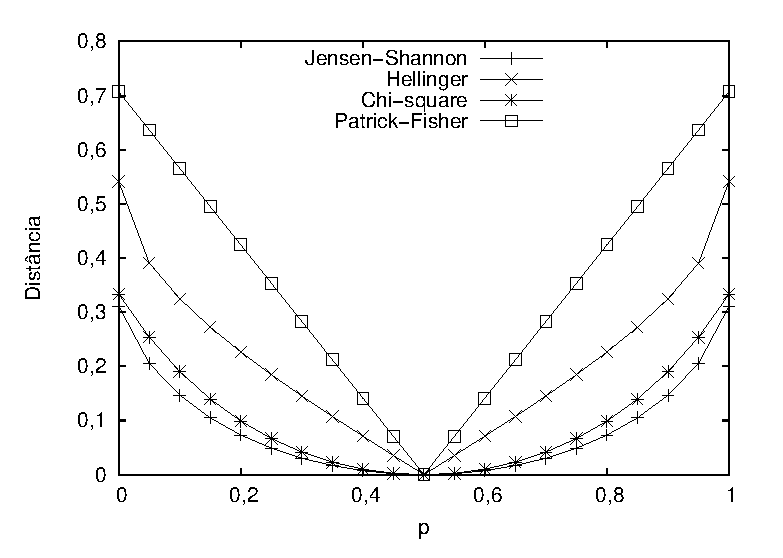
\includegraphics[width=0.75\textwidth]{graph2.eps}
\end{figure}

%\subsection{Divergente de Rényi}
O divergente de Rényi generaliza algumas das medidas de divergência apresentadas até então.

%$D_{\alpha}(p,q) =\frac{1}{\alpha-1}\log{\sum\limits_{i = 1}^{n}{p_i^{\alpha}q_i^{1-\alpha}}}$

%\subsection{Chernoff}
%$\displaystyle D_C(p,q) = - \min_{0<\alpha<1}{log{\sum\limits_{i=1}^{n}{p_i^{\alpha}q_i^{1-\alpha}}}}$

%\subsection{Bhattacharyya}
%$D_{B}(p,q) = -2log{\sum\limits_{i = 1}^{n}{\sqrt{p_{i}q_{i}}}}$

%\subsection{Hellinger}
%$D_{H}=\frac{1}{\sqrt{2}}\sqrt{\sum\limits_{i = 1}^{n}{(\sqrt{p_{i}}-\sqrt{q_{i}})^2}}$

\begin{comment}

The concept of fractal, introduced by Mandelbrot \citep{Mandelbrot:2000}, is closely related to self-similarity or scaling of a shape. Moreover, it encompasses the notion of fractional dimension.  Actually, fractal dimension and \emph{MFD} are well-known methods to estimate shape complexity \citep{Backes:2012}. Shape complexity is an important concept in shape analysis that informs how much space a shape occupies \cite{Costa:2009}. \emph{MFD} estimates shape complexity through a curve that represents changes in the complexity as the shape visualization scale varies \cite{Florindo:2012}. 

%and for feature extraction of biological forms %\citep{Rossatto:2011}.  In fact, it quantifies the %self-similarity of a shape.

% quantifica a aspereza ou rugosidade de uma forma \citep{Schroreder:1996}.\\

%Uma das caracter\'isticas das formas fractais \'e a sua auto-similaridade \citep{Schroreder:1996}. Isso significa que uma forma, tanto em escalas menores como maiores, \'e constitu\'ida por um mesmo conjunto de primitivas $D_f$.\\

%Qualquer forma auto-similar pode ser dividida em $N$ partes auto-similares, ou seja, c\'opias menores que sejam escalonadas por um fator $b$, atrav\'es da equa\c c\~ao:\\

%\begin{equation}
%D_{f} = \frac{\log{N}}{\log{\frac{1}{b}}}.
%\label{eq:dfc}
%\end{equation}

%Esse descritor pode ser construído a partir do método de Bouligand-Minkowski de estimação da dimensão fractal ($D_f$) \citep{Costa:2009}. Utilizado em \citep{Florindo:2012} e \citep{Backes:2012}, o referido método aplica dilatações exatas à  forma analisada tendo como elemento estruturante uma região circular de raio $r > 0$. O coeficiente angular da interpolação linear da curva $\log{A(r)}$ versus $\log{r}$ é utilizado como uma estimativa da $D_f$:

In this paper, the Minkowski-Bouligand method estimates the fractal dimension ($D_f$) \citep{Costa:2009} and hence the \emph{MFD} descriptor. This estimation method dilates the shape under analysis  using a disk structuring element of radius $ r>0 $, successively. The slope of the linear interpolation of the curve $\log{A(r)}$ versus $\log{r}$ provides the $D_f$ estimation, given by: 

\begin{equation}
D_f = 2 - \lim_{r \to 0}  \frac{\log{A(r)}}{\log{r}}.
\label{eq:df}
\end{equation}
%O cálculo da MFD decorre do calculo da derivada da curva log-log, obtida a partir da equação \ref{eq:df}, para diferentes valores de raios $r$:
Then, the derivative of th log-log curve for $N$ discrete values of radii $r_i>0$ gives 

\begin{equation}
MFD = \big(D_f(t_1)\text{, }D_f(t_2)\text{, }\ldots\text{ , }D_f(t_N)\big), 
\label{eq:dfm}
\end{equation}

\noindent where  $D_f(t) = 2 - \frac{du(t)}{dt}$, $t = \log{r}$ and $u(t) = \log{A(t)}$.

\end{comment}

\section{Entropia multiescala}

No Capítulo \ref{chap:contour} mostramos como se obtém a curvatura multiescala como uma assinatura do contorno de uma forma. No mesmo capítulo apresentamos um descritor multiescala construído a partir da versão discreta dessa assinatura, mais especificamente a energia de dobramento multiescala. Aqui propomos um descritor multiescala a partir dessa mesma assinatura, mas explorando os conceitos de entropia diferencial.

Para se obter o descritor multiescala proposto é necessário estimar as funções densidade de probabilidade do sinal da curvatura em diferentes escalas. \citeonline{Principe:2010:ITL:1855180} sugere a janela de Parzen \cite{Webb:2002} como uma técnica conveniente para se estimar funções densidade de probabilidade, sendo essa técnica a empregada para realizar tais estimativas neste trabalho.
 
 Para uma dada escala $\sigma'$, temos a curvatura amostrada em $M$ valores como sendo $K[t,\sigma'] = \{K[1,\sigma']\text{, }K[2,\sigma']\text{, }\ldots\text{, }K[M,\sigma']\}$. A função densidade de probabilidade dessa função, estimada pela janela de Parzen, é dada por \cite{Webb:2002}:  
 
\begin{equation}\label{eq:parzen}
p_{\sigma'}(k) = \frac{1}{bM}\sum\limits_{i=1}^M\Psi(\frac{k - K[i,\sigma']}{b})\text{,}
\end{equation}

sendo $\Psi(z) = \frac{1}{\sqrt{2\pi}}\exp{-\frac{z^2}{2}}$ a função de janela e $b$ a sua largura de banda.

No processo de estimação através dessa técnica a escolha do parâmetro largura de banda é crítica, pois esse altera o grau de suavização da curva de densidade obtida. Valores elevados desse parâmetro tendem a suavizar em demasia a curva de densidade estimada acarretando em perda de detalhes importantes. Por outro lado, valores pequenos resultam em densidades estimadas com mais detalhes, porém mais ruidosa. Assim, é importante estabelecer um critério para escolha do parâmetro de largura de banda para que se tenha uma boa estimativa da função densidade de probabilidade. Adotamos neste trabalho o método proposto por Silverman \cite{silverman:1986}. Esse método, que determina uma escolha ótima de largura de banda, assume que a distribuição de probabilidade dos dados é normal e que a janela utilizada é gaussiana.

A largura de banda pelo método de Silverman é dada por \cite{silverman:1986}

\begin{equation}
b = \big(\frac{4\hat{\sigma}^5}{3n}\big)^\frac{1}{5}\text{,}
\end{equation}

sendo $\hat{\sigma}$ o desvio padrão e $n$ o número das amostras utilizadas no processo de estimação. 

Temos o cálculo da entropia diferencial da curvatura multiescala na escala $\sigma'$ aplicando o resultado obtido da Equação \ref{eq:parzen} na Equação \ref{eq:difent}, ou seja:

\begin{equation}\label{eq:desc_entropia}
h\big(K[t,\sigma']\big) = -\int_{-K_{min}}^{K_{max}}p_{\sigma'}(k)\log{p_{\sigma'}(k)}dk\text{, }
\end{equation}

sendo a integral calculada através do método numérico de integração de Simpson e os limites de integração $K_{min}$ e $K_{max}$ os valores máximos e mínimos da curvatura multiescala na escala $\sigma'$.

O descritor obtido a partir da equação \ref{eq:desc_entropia} apresenta propriedades de invariância a translação e a rotação. Isso porque a translação da forma não afeta o sinal da curvatura. Embora a rotação desloque em fase o sinal da curvatura, como ilustra a figura \ref{fig:curv_scale_rot}a, esse deslocamento não interfere na função densidade de probabilidade estimada, e portanto não interfere no cálculo do descritor.

Porém, o descritor não apresenta invariância a mudança de escala da forma. Isso porque tal mudança reflete em escala no sinal de curvatura (figura \ref{fig:curv_scale_rot}b), o que interfere na função densidade de probabilidade estimada, e portanto no cálculo do descritor.

Consegue-se a invariância do descritor à mudança de escala utilizando o perímetro da forma ($L_{\sigma'}$) como fator de normalização. Desta forma, aplicando a  propriedade da equação \ref{eq:escala_entropia}, temos a versão do descritor invariante a mudança de escala:

\begin{equation}\label{eq:entropia_inv}
\hat{h}\big(K(t,\sigma')\big) = -\int_{-K_{min}}^{K_{max}} p_{\sigma'}(k)\log{p_{\sigma'}(k)}dk+\log{L_{\sigma'}}\text{.}
\end{equation}

\begin{figure}[]
\caption{\label{fig:curv_scale_rot}Efeitos da rotação e da mudança de escala das formas sobre a curvatura.}
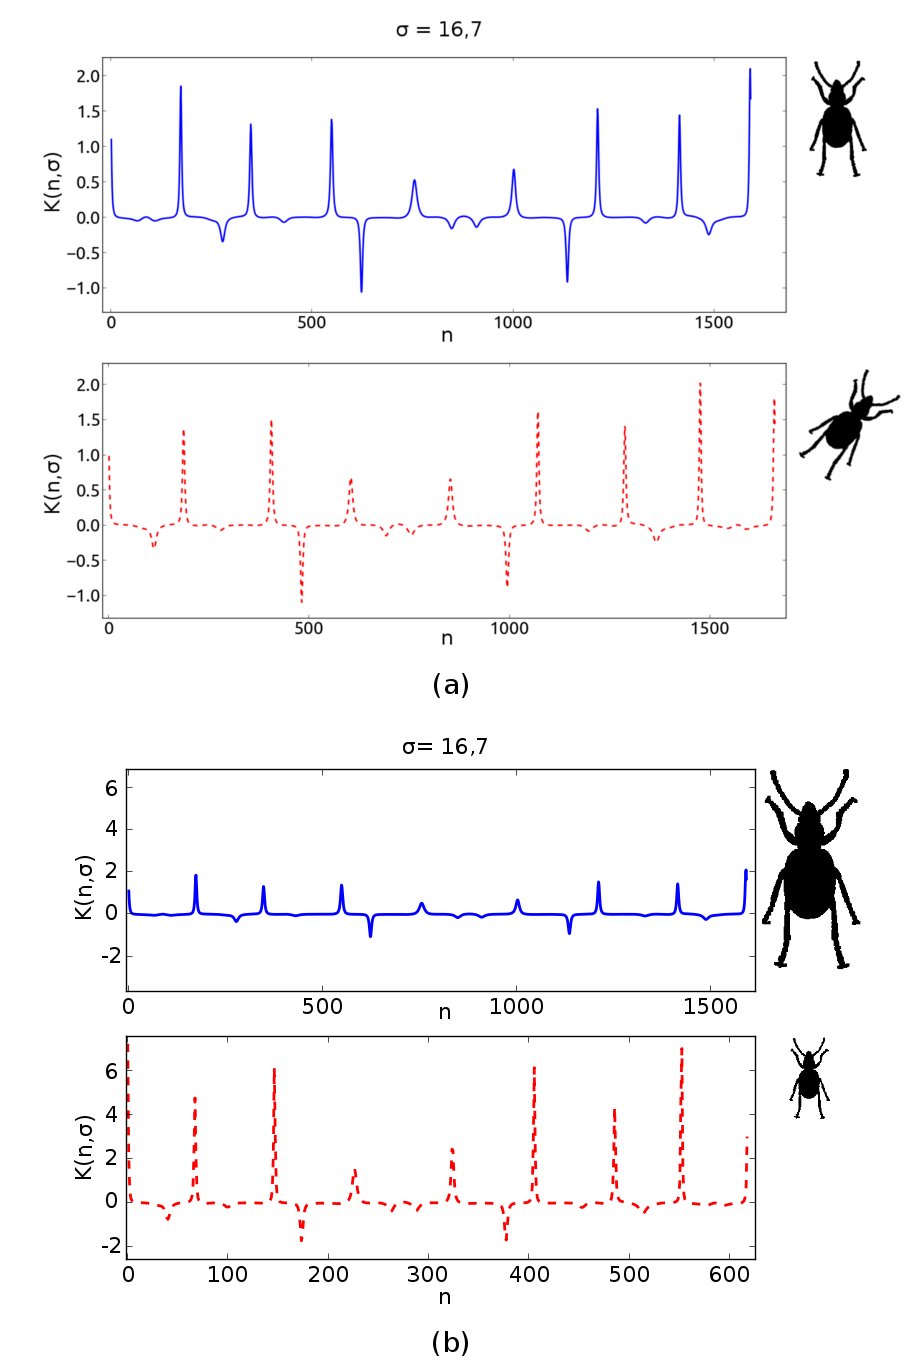
\includegraphics[width=\textwidth]{curvatura_scale_rot.png}
\end{figure}

As figuras \ref{fig:entropia_inv}a e \ref{fig:entropia_inv}b ilustram o descritor entropia diferencial da curvatura multiescala, calculado para duas formas idênticas, em diferentes escalas. Na figura \ref{fig:entropia_inv}a o cálculo foi realizado através da equação \ref{eq:entropia_inv} e o descritor mostrou invariância à mudança de escala da forma. Já na figura \ref{fig:entropia_inv}b o cálculo foi realizado a partir da equação \ref{eq:desc_entropia} e o descritor não apresentou invariância à escala da forma.

A figura \ref{fig:entropia_inv}c ilustra a invariância do descritor à rotação da forma. Nesse caso, o cálculo foi realizado a partir da equação \ref{eq:entropia_inv}.

\begin{figure}[]
\caption{\label{fig:entropia_inv}Efeitos da rotação e da mudança de escala das formas sobre o descritor entropia multiescala.}
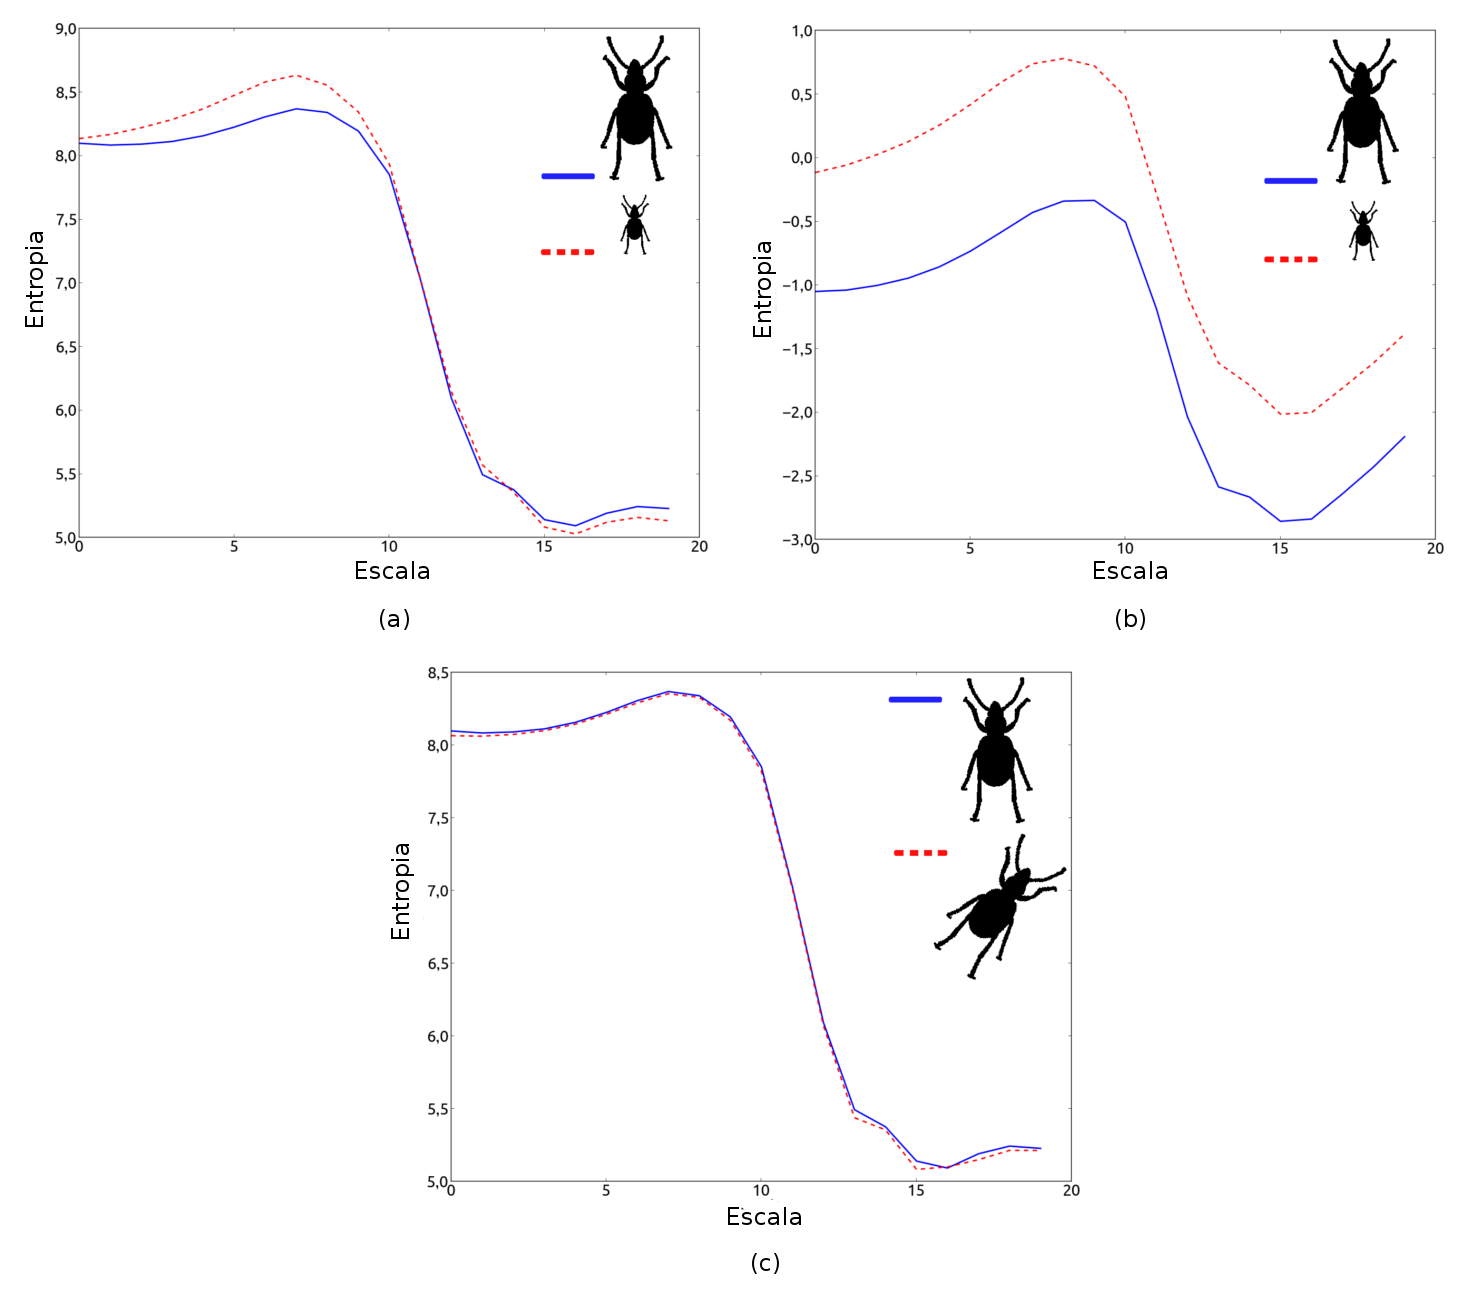
\includegraphics[width=\textwidth]{inv_entropia.png}
\end{figure}

\section{Medidas de divergência em similaridade de formas \label{Sec:divergente}}

\begin{figure}[]
  \caption{\label{fig:metodo_distancia} Método para avaliação da similaridade entre duas formas A e B através de medidas de divergência e histogramas das assinaturas do contorno das formas.}
  \centering
  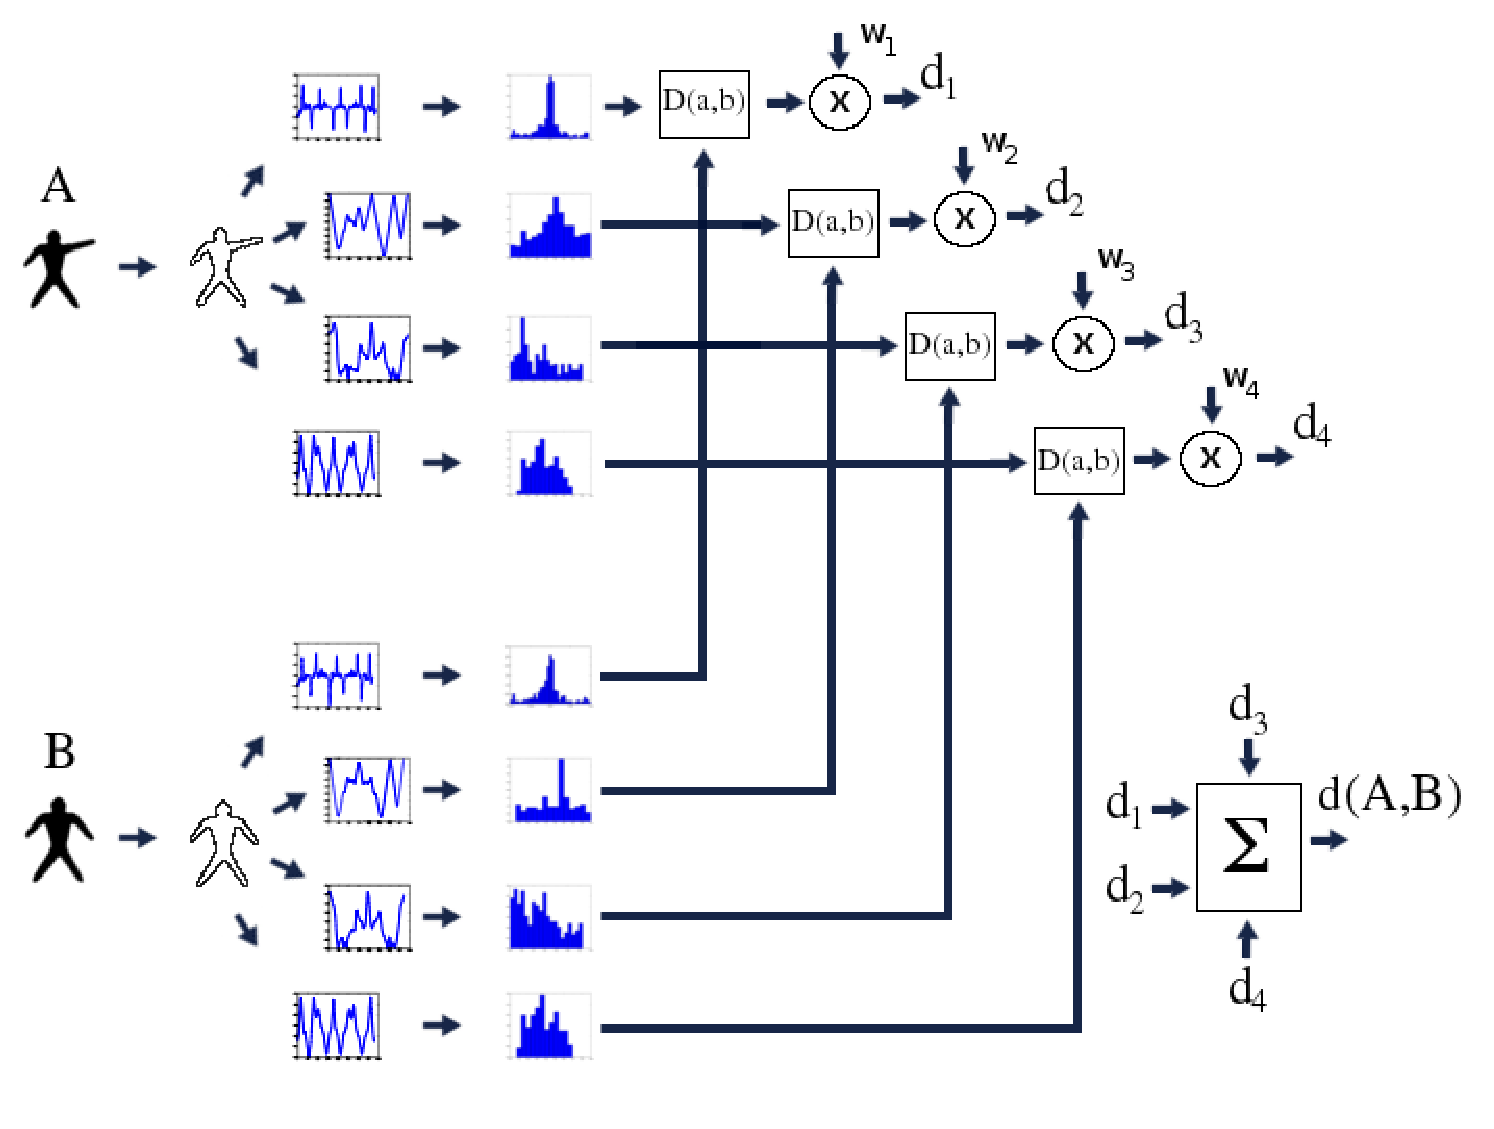
\includegraphics[width=0.85\textwidth]{figura_metodo.eps}
\end{figure}

O método proposto para a avaliação de similaridade entre duas formas A e B, ilustrado na Figura \ref{fig:metodo_distancia},  combina medidas de divergência com assinaturas do contorno das
formas. Uma vez extraído o contorno são calculadas as quatro assinaturas apresentadas na Seção \ref{sec:Assinatura} do Capítulo \ref{chap:contour}: curvatura \cite{149591,Costa:2009}, sequência de ângulos (AS) \cite{Fotopoulou:2013}, distância ao centróide (CD) \cite{Costa:2009} e invariante integral de área (AII) \cite{Manay:2006}. Então, estimam-se as distribuições de probabilidade dessas assinaturas através de histogramas. Um ponto considerado na determinação dos histogramas é o ajuste dos parâmetros utilizados na estimação das distribuições, que são o número de intervalos (bins) e a faixa de valores. Um número de intervalos grande torna a estimação sensível a ruído, enquanto um número pequeno desse parâmetro resulta em uma descrição com poder de discriminação pobre. Já a má escolha da faixa de valores resulta em perda de informação na descrição, o que também degrada o poder de discriminação.  Assim, a faixa de valores foi padronizada normalizando-se as assinaturas das formas, enquanto os números de intervalos (um parâmetro para cada assinatura) foram obtidos por otimização para maximizar o desempenho do descritor, conforme o método da Seção ??. 

Finalmente, as medidas de divergência $D(a,b)$ entre os histogramas correspondentes das formas A e B são calculados, resultando em quatro medidas de dissimilaridade, uma para cada par de assinaturas ($d_{1}$, $d_{2}$, $d_{3}$ e $d_{4}$), sendo a medida de dissimilaridade final $d(A,B) = d_{1}+d_{2}+d_{3}+d_{4}$. Cabe aqui mencionar que, por ser uma medida de dissimilaridade, quanto menor o valor de $d(A,B)$ maior a similaridade entre as formas $A$ e $B$. 

Realizou-se experimentos de recuperação de formas para avaliar o qualidade do método em questão para diferentes funções de divergência.


